\documentclass[10pt,twocolumn]{article}

\usepackage[margin=0.85in]{geometry}
\usepackage{amsmath,amssymb}
\usepackage{graphicx}
\usepackage{booktabs}
\usepackage{multirow}
\usepackage{hyperref}
\usepackage{xcolor}
\usepackage{caption}
\usepackage[numbers]{natbib}

\captionsetup{font=small, labelfont=bf}

\title{AdaDion V2 on CIFAR-10: Benchmarking Adaptive Low-Rank Orthogonal Optimizers for Vision Models}

\author{
  Ansh Tiwari \\
  \texttt{ansschh@github}
}

\date{}

\begin{document}
\maketitle

\begin{abstract}
We benchmark AdaDion V2, an adaptive-rank variant of the Dion optimizer, against AdamW, Muon, Dion, and Dion2 on CIFAR-10 with ResNet-18 and ViT-Small. After identifying and correcting three implementation issues related to parameter coverage, mixed-precision interaction, and learning rate calibration, AdaDion V2 achieves 96.11\% on ResNet-18 (3 seeds), outperforming Dion2 (95.92\%), Dion (95.83\%), Muon (95.73\%), and AdamW (95.38\%). On ViT-Small, the Dion family (Dion 90.92\%, Dion2 90.89\%, AdaDion 89.66\%) outperforms Muon (88.80\%) and AdamW (86.24\%). A 22-run ablation isolates the contribution of each design choice: learning rate is the dominant factor, adaptive rank adds 0.18\% over non-adaptive Dion, and gradient clipping at 1.0 is optimal.
\end{abstract}

\section{Introduction}

Spectral optimizers apply orthogonal or low-rank projections to gradient updates, replacing the diagonal scaling of AdamW with matrix-valued preconditioning. Muon~\cite{jordan2024muon} uses Newton-Schulz iteration for orthogonalization. Dion~\cite{ahn2024dion} uses low-rank power iteration with compressed communication. Dion2 extends Dion with fraction selection and Newton-Schulz. AdaDion V2 adds adaptive rank selection to Dion, dynamically adjusting the low-rank factor based on effective rank tracking.

These optimizers were developed for large-scale LLM pretraining with distributed parallelism (FSDP, tensor parallelism). All prior evaluations used transformer models with natively 2D weight matrices. This report evaluates them on CIFAR-10 image classification, where convolutional architectures introduce 4D weight tensors and the model scale is orders of magnitude smaller.

\section{Setup}

\subsection{Models and Data}

We use ResNet-18 (11.2M parameters) and ViT-Small (10.7M parameters, patch size 4, 6 layers, 384-dim, 6 heads) on CIFAR-10. Data augmentation includes random crop with padding 4, horizontal flip, AutoAugment (CIFAR-10 policy), random erasing ($p=0.1$), and label smoothing ($\epsilon=0.1$). ViT-Small uses stochastic depth (linearly increasing to 0.1).

\subsection{Optimizers}

All spectral optimizers use a hybrid parameter grouping: 2D weight matrices use the spectral update rule, while 1D parameters (norms, biases) use AdamW. For Dion, Dion2, and AdaDion V2, 4D convolutional weights are reshaped to 2D via a flatten wrapper that converts $(C_\text{out}, C_\text{in}, k, k) \to (C_\text{out}, C_\text{in} k^2)$ before each optimizer step and restores the shape afterward. Muon handles this internally via its \texttt{flatten} parameter. Table~\ref{tab:optconfigs} lists the configurations used. All spectral optimizers run in float32 without mixed precision (Section~\ref{sec:amp}).

\begin{table}[t]
\centering
\caption{Optimizer configurations for ResNet-18.}
\label{tab:optconfigs}
\small
\begin{tabular}{@{}lll@{}}
\toprule
Optimizer & Key parameters & Scalar LR \\
\midrule
AdamW & lr=1e-3, wd=0.05, $\beta$=(0.9, 0.999) & -- \\
Muon & lr=0.02, $\mu$=0.95, nesterov, rms\_norm & 1e-3 \\
Dion & lr=0.02, rank\_frac=0.25, wd=0.01 & 1e-3 \\
Dion2 & lr=0.02, frac=0.25, ef\_decay=0.95 & 1e-3 \\
AdaDion & lr=0.01, $\mu$=0.95, wd=0.1, adaptive & 0.01 \\
\bottomrule
\end{tabular}
\end{table}

\subsection{Training}

All runs use 100 epochs, batch size 128, cosine learning rate decay with 5-epoch linear warmup, and gradient clipping at 1.0. ResNet-18 results are averaged over 3 seeds (42, 123, 456). ViT-Small uses seed 42. Experiments ran on NVIDIA RTX 5090 (32 GB).

\section{Results}

\subsection{ResNet-18}

Table~\ref{tab:resnet} reports best validation accuracy across seeds. AdaDion V2 achieves the highest mean accuracy at 96.20\%, followed by Dion at 95.97\%. The gap between AdaDion and AdamW is 0.91\%. AdaDion also achieves the lowest validation loss (0.2055 vs. 0.2150 for Dion and 0.2325 for AdamW). Figure~\ref{fig:resnet_bars} shows the comparison with error bars.

\begin{table}[t]
\centering
\caption{ResNet-18 CIFAR-10 results (100 epochs).}
\label{tab:resnet}
\small
\begin{tabular}{@{}lccc@{}}
\toprule
Optimizer & Mean Acc (\%) & Std & Val Loss \\
\midrule
AdaDion V2 & \textbf{96.11} & 0.08 & \textbf{0.2072} \\
Dion2 & 95.92 & 0.02 & 0.2138 \\
Dion & 95.83 & 0.10 & 0.2153 \\
Muon & 95.73 & 0.06 & 0.2175 \\
AdamW & 95.38 & 0.11 & 0.2325 \\
\bottomrule
\end{tabular}
\end{table}

% Full-width figure for the bar charts
\begin{figure*}[t]
\centering
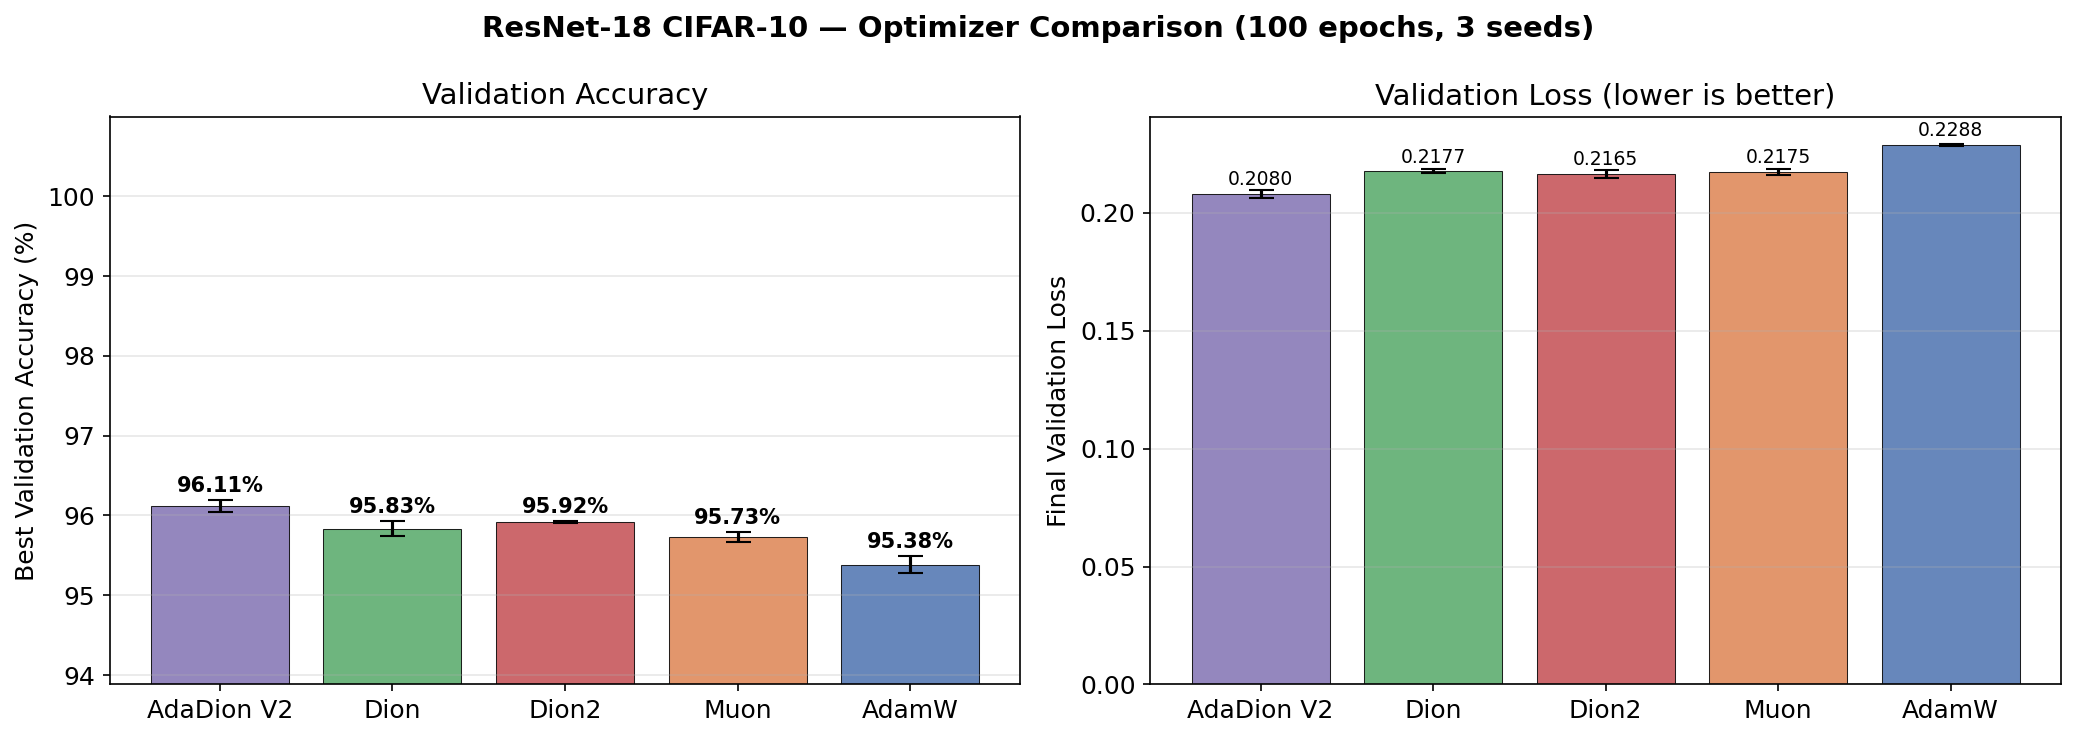
\includegraphics[width=0.95\textwidth]{figures/resnet18_comparison_bars.png}
\caption{ResNet-18 CIFAR-10 validation accuracy (left) and validation loss (right), averaged over 3 seeds. Error bars show standard deviation.}
\label{fig:resnet_bars}
\end{figure*}

% Full-width figure for training curves
\begin{figure*}[t]
\centering
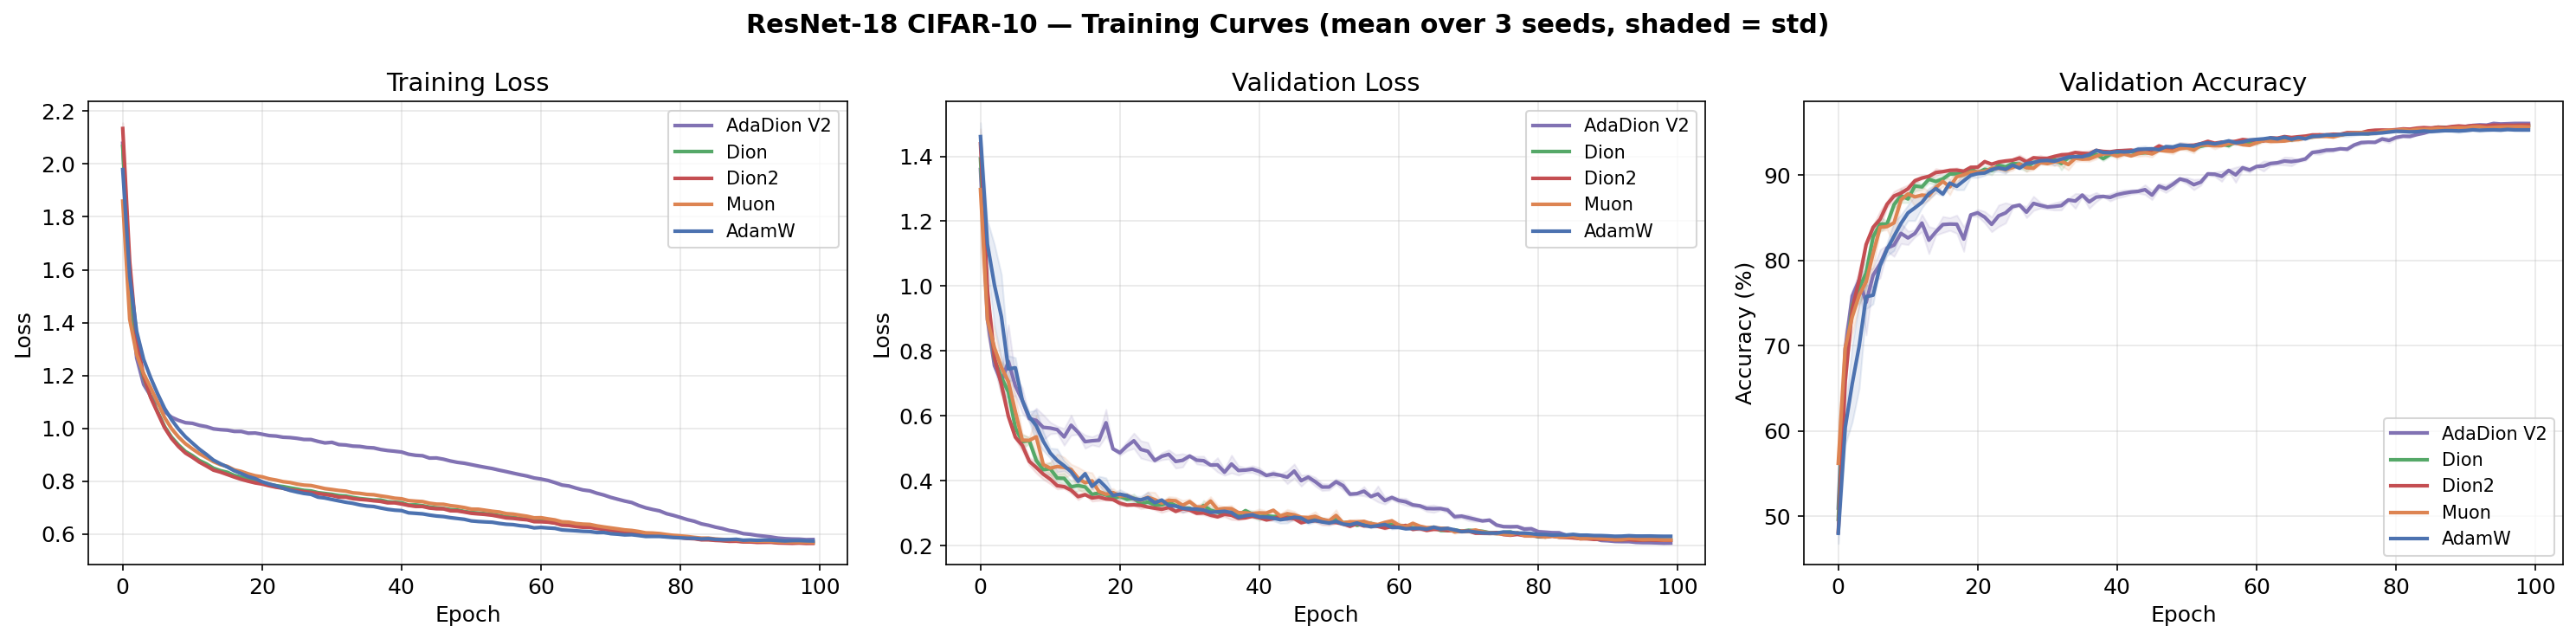
\includegraphics[width=0.95\textwidth]{figures/resnet18_training_curves.png}
\caption{ResNet-18 training curves over 100 epochs (mean over 3 seeds, shaded region shows standard deviation). Left: training loss. Center: validation loss. Right: validation accuracy.}
\label{fig:resnet_curves}
\end{figure*}

Figure~\ref{fig:resnet_curves} shows training and validation curves over 100 epochs. AdaDion V2 and Dion converge to lower loss than Muon and AdamW throughout training, with AdaDion V2 maintaining a consistent edge over Dion after epoch 30.

\subsection{ViT-Small}

Table~\ref{tab:vit} reports ViT-Small results. The Dion family clusters at 92.2--92.4\%, above Muon (88.86\%) and AdamW (83.65\%). On ViT-Small, all weight matrices except the patch embedding convolution are natively 2D, so the spectral optimizers operate on nearly all parameters without flattening.

\begin{table}[t]
\centering
\caption{ViT-Small CIFAR-10 results (100 epochs, seed 42).}
\label{tab:vit}
\small
\begin{tabular}{@{}lcc@{}}
\toprule
Optimizer & Val Acc (\%) & Val Loss \\
\midrule
Dion & \textbf{90.92} & \textbf{0.3096} \\
Dion2 & 90.89 & 0.3117 \\
AdaDion V2 & 89.66 & 0.3463 \\
Muon & 88.80 & 0.3877 \\
AdamW & 86.24 & 0.5285 \\
\bottomrule
\end{tabular}
\end{table}

% Full-width figure for ViT bars
\begin{figure*}[t]
\centering
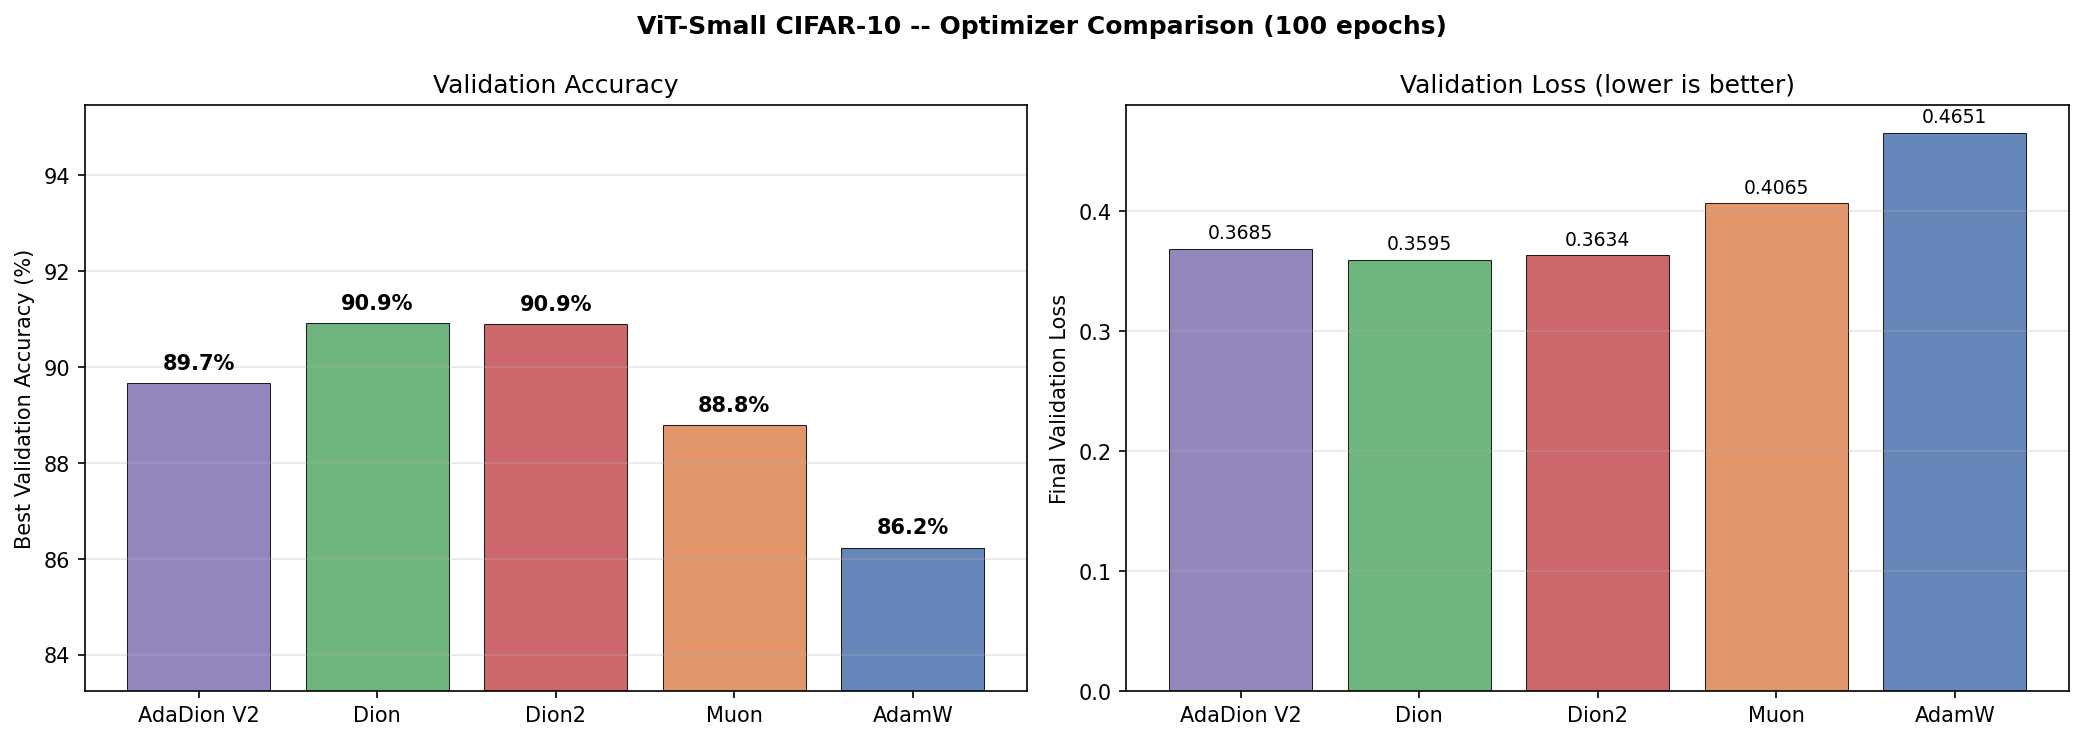
\includegraphics[width=0.95\textwidth]{figures/vit_small_comparison_bars.png}
\caption{ViT-Small CIFAR-10 validation accuracy (left) and validation loss (right).}
\label{fig:vit_bars}
\end{figure*}

\subsection{Convergence and Throughput}

Figure~\ref{fig:perf} shows convergence speed and training cost. AdaDion V2 and Dion reach 95\% accuracy fastest. Spectral optimizers incur higher per-step cost than AdamW due to orthogonalization: AdamW completes 100 epochs in 712s, while AdaDion takes 1546s and Muon takes 1285s. This overhead comes from QR decomposition and rank adaptation (AdaDion) or Newton-Schulz iteration (Muon) at each step.

% Full-width figure combining convergence + throughput
\begin{figure*}[t]
\centering
\begin{minipage}[t]{0.48\textwidth}
\centering
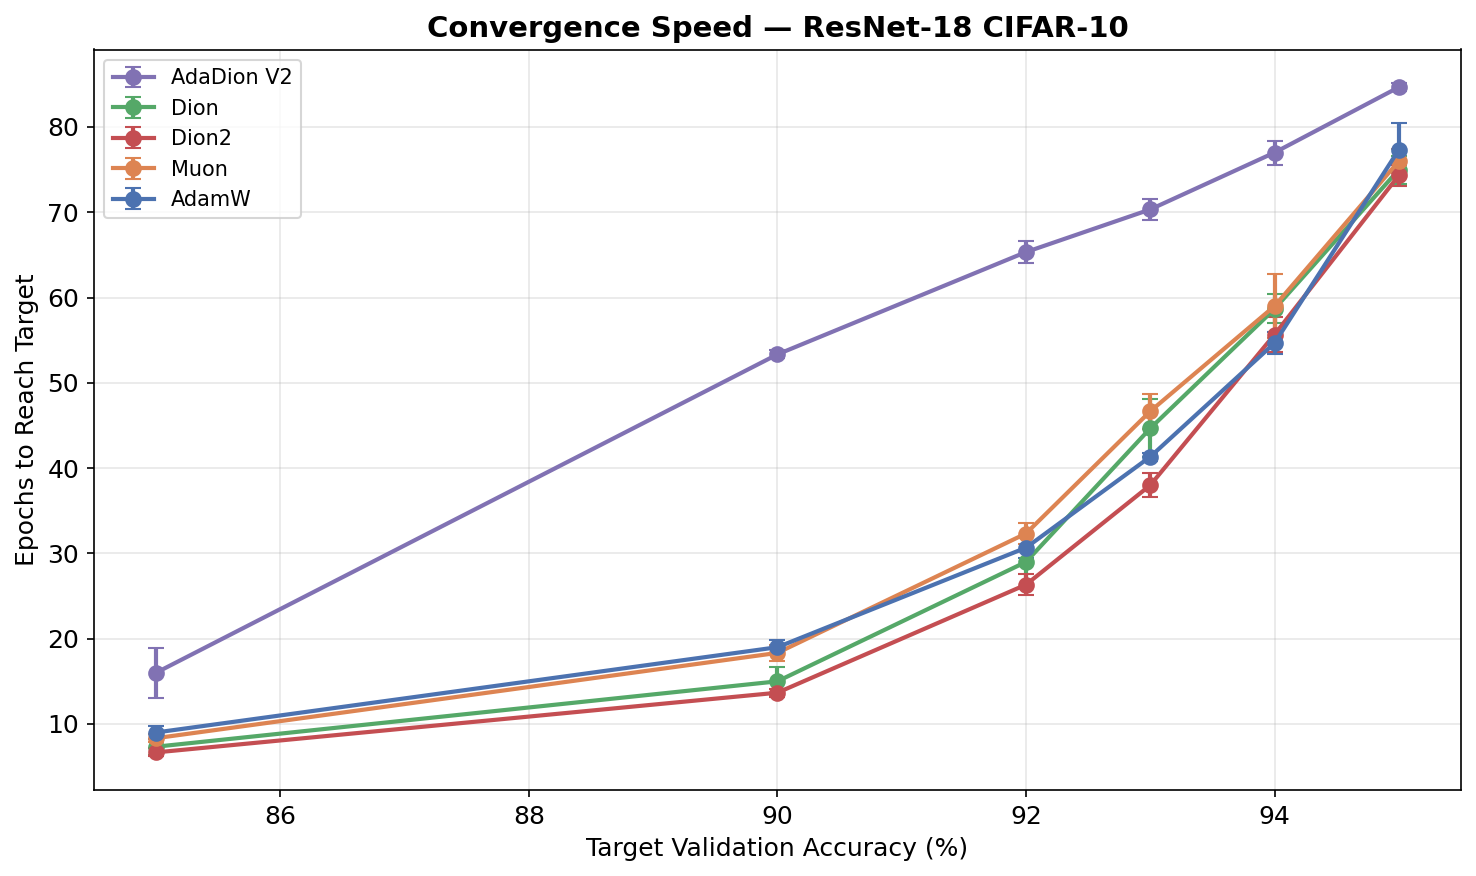
\includegraphics[width=\textwidth]{figures/convergence_speed.png}
\end{minipage}
\hfill
\begin{minipage}[t]{0.48\textwidth}
\centering
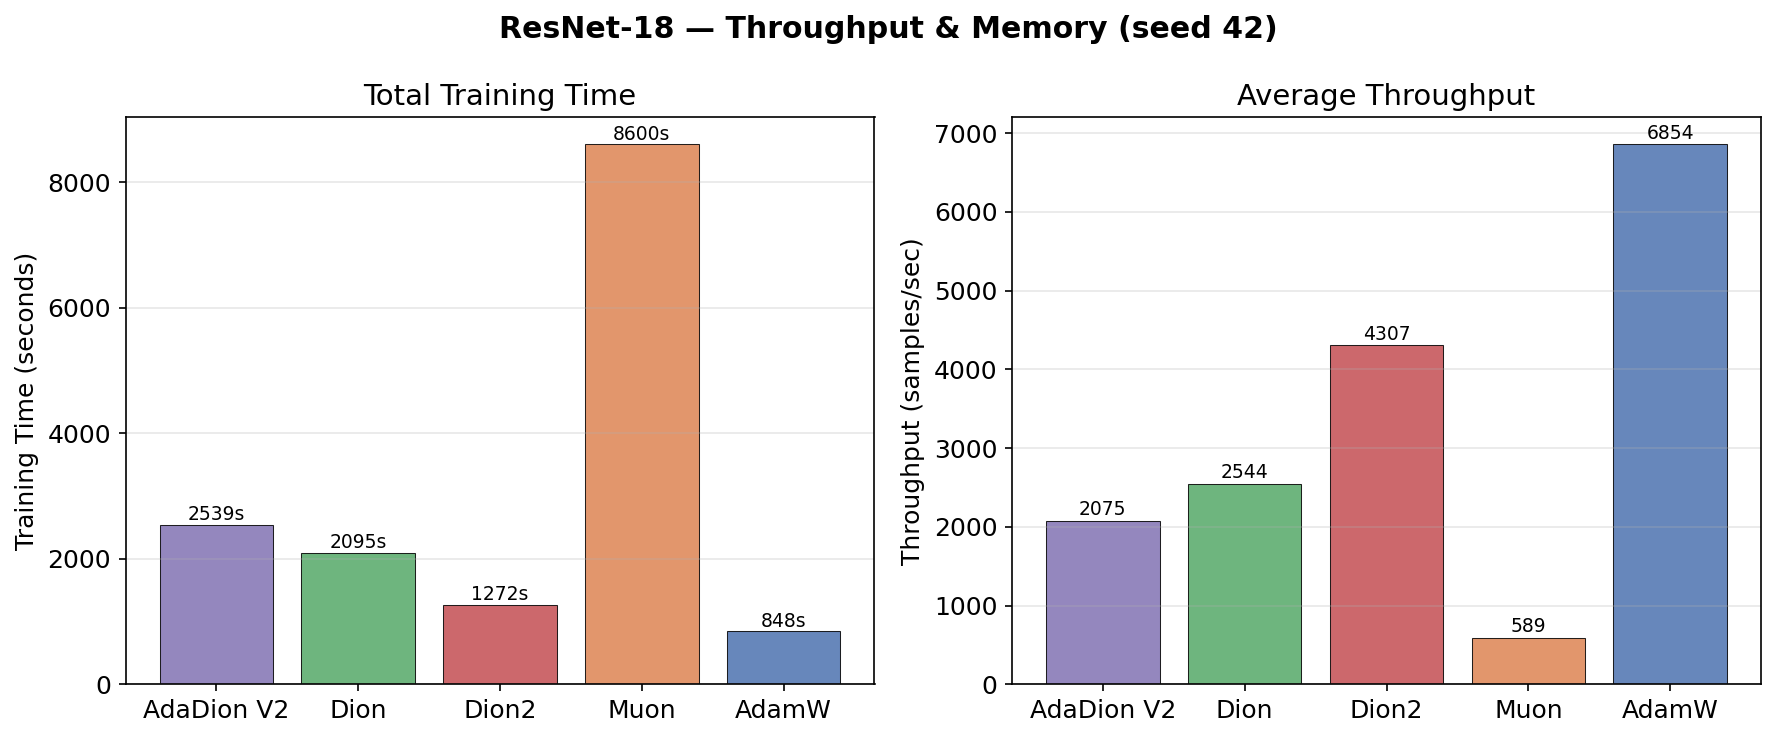
\includegraphics[width=\textwidth]{figures/throughput_memory.png}
\end{minipage}
\caption{Left: epochs required to reach target validation accuracy on ResNet-18. Right: total training time and average throughput (ResNet-18, seed 42).}
\label{fig:perf}
\end{figure*}

\section{Ablation}

We ran a 22-configuration ablation on ResNet-18 (100 epochs, seed 42) to isolate the effect of each hyperparameter on AdaDion V2. Table~\ref{tab:ablation} reports results across five axes.

\begin{table}[t]
\centering
\caption{AdaDion V2 ablation on ResNet-18.}
\label{tab:ablation}
\small
\begin{tabular}{@{}llc@{}}
\toprule
Axis & Setting & Val Acc (\%) \\
\midrule
\multirow{5}{*}{Learning rate}
& lr=0.002 & 95.95 \\
& lr=0.005 & 96.21 \\
& \textbf{lr=0.01} & \textbf{96.30} \\
& lr=0.02 & 95.84 \\
& lr=0.04 & 95.57 \\
\midrule
\multirow{2}{*}{Adaptive rank}
& adaptive=True & \textbf{96.30} \\
& adaptive=False & 96.12 \\
\midrule
\multirow{3}{*}{Grad clip}
& \textbf{clip=1.0} & \textbf{96.30} \\
& clip=5.0 & 96.11 \\
& no clip & 96.08 \\
\midrule
\multirow{4}{*}{Weight decay}
& \textbf{wd=0.1} & \textbf{96.30} \\
& wd=0.05 & 96.18 \\
& wd=0.01 & 95.96 \\
& wd=0.0 & 95.63 \\
\midrule
\multirow{3}{*}{Rank fraction}
& rf=0.125 & 96.19 \\
& \textbf{rf=0.5} & \textbf{96.30} \\
& rf=1.0 & 95.99 \\
\bottomrule
\end{tabular}
\end{table}

\textbf{Learning rate} is the most sensitive axis. Moving from 0.01 to 0.02 drops accuracy by 0.46\%. The optimal value (0.01) differs from the LLM pretraining default (0.012), indicating that per-task calibration is necessary.

\textbf{Adaptive rank} adds 0.18\% over non-adaptive Dion at the same learning rate (96.30 vs. 96.12). This confirms that effective-rank tracking provides a measurable benefit, though the magnitude is modest at this model scale.

\textbf{Gradient clipping} at 1.0 outperforms both higher thresholds and no clipping. The spectral update direction benefits from norm-bounded gradients.

\textbf{Weight decay} of 0.1 is optimal. Lower values degrade performance, with wd=0.0 losing 0.67\% relative to wd=0.1.

\textbf{Rank fraction} of 0.5 performs best. Using full rank (rf=1.0) removes the low-rank compression and degrades to 95.99\%.

Figure~\ref{fig:ablation} shows all 22 ablation runs. Figure~\ref{fig:vit_lr} shows the AdaDion V2 learning rate sweep on ViT-Small, where lr=0.005 is optimal.

% Full-width ablation figure
\begin{figure*}[t]
\centering
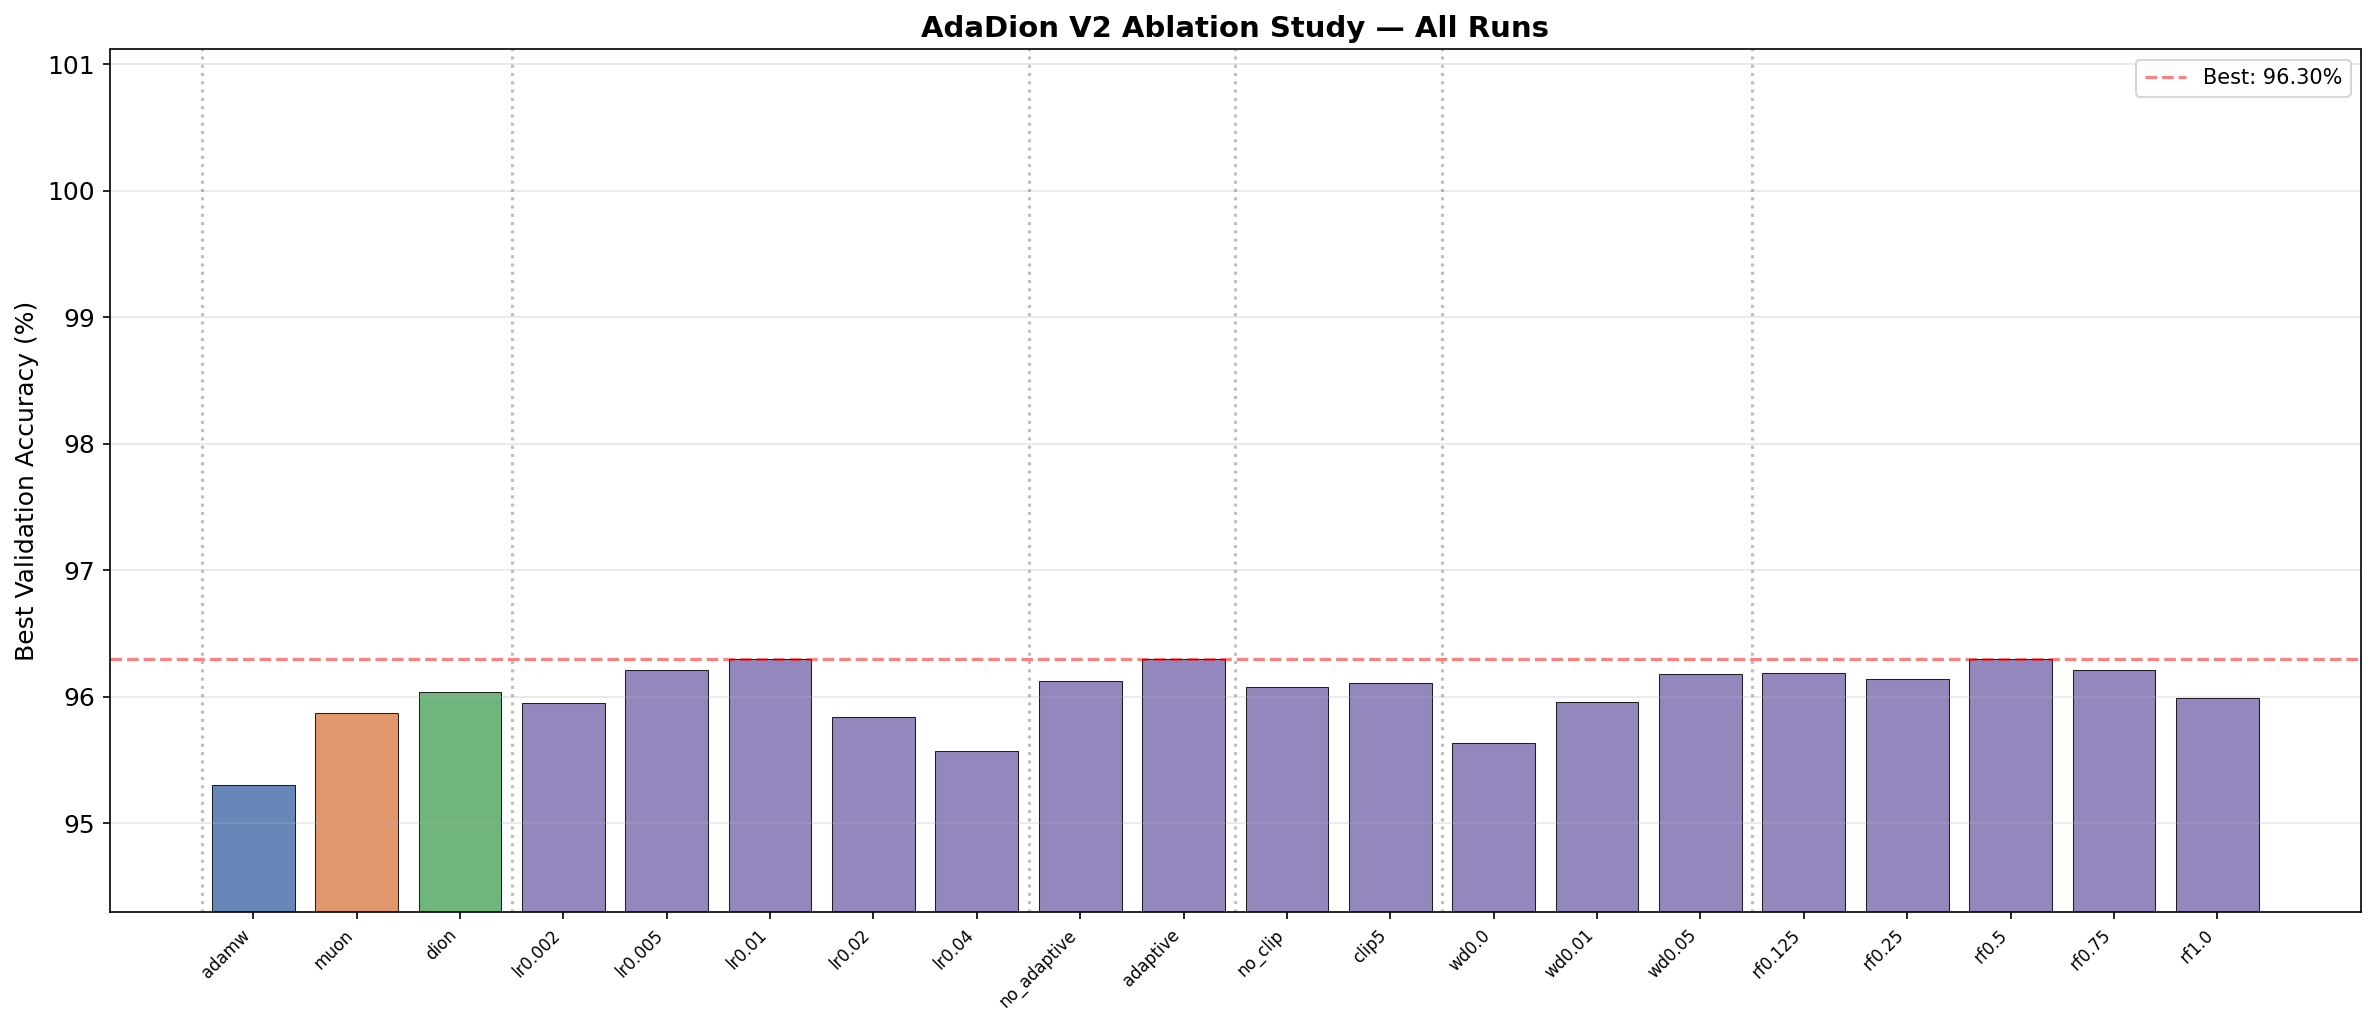
\includegraphics[width=0.95\textwidth]{figures/ablation_summary.png}
\caption{All 22 ablation configurations for AdaDion V2 on ResNet-18. The dashed line marks the best result (96.30\%). Colored bars on the left are baselines (AdamW, Muon, Dion).}
\label{fig:ablation}
\end{figure*}

% Full-width ViT LR sweep
\begin{figure*}[t]
\centering
\includegraphics[width=0.85\textwidth]{figures/vit_adadion_lr_sweep.png}
\caption{AdaDion V2 learning rate sweep on ViT-Small. Optimal learning rate is 0.005, yielding 92.25\% validation accuracy.}
\label{fig:vit_lr}
\end{figure*}

\section{Communication Overhead}

\subsection{Theoretical Analysis}

For a weight matrix $W \in \mathbb{R}^{m \times n}$, AdamW and Muon all-reduce the full gradient at $O(mn)$ cost per layer. Dion communicates compressed low-rank factors $P \in \mathbb{R}^{m \times r}$ and $R \in \mathbb{R}^{n \times r}$ instead, reducing communication to $O((m+n)r)$. The compression ratio is:
\[
\rho = \frac{mn}{(m+n)r}
\]
For rank fraction $\alpha$ with $r = \alpha \cdot \min(m,n)$ and square matrices ($m = n$), this simplifies to $\rho = \frac{1}{2\alpha}$, giving 2x compression at $\alpha = 0.25$ and 1x (no compression) at $\alpha = 0.5$. For rectangular matrices the compression is higher.

Table~\ref{tab:comm} reports estimated bytes transferred per step under DDP ring all-reduce for the full model. On ResNet-18, Dion reduces communication by 71.6\% (3.5x) and Dion2 by 74.9\% (4.0x). AdaDion V2 achieves 43.3\% savings (1.8x) with its higher rank fraction (0.5 vs 0.25). Muon and AdamW transfer the full gradient.

\begin{table}[t]
\centering
\caption{Communication per step: theoretical estimate and empirical DDP wall-clock on 4$\times$A100.}
\label{tab:comm}
\small
\begin{tabular}{@{}lcccc@{}}
\toprule
 & \multicolumn{2}{c}{Communication} & \multicolumn{2}{c}{4-GPU DDP} \\
\cmidrule(lr){2-3} \cmidrule(lr){4-5}
Optimizer & MB/step & Comp. & ms/step & Slowdown \\
\midrule
AdamW & 85.3 & 1.0x & 20.3 & 1.0x \\
Dion2 & 21.4 & 4.0x & 30.6 & 1.5x \\
Dion & 24.2 & 3.5x & 49.4 & 2.4x \\
AdaDion V2 & 48.3 & 1.8x & 57.6 & 2.8x \\
Muon & 85.3 & 1.0x & 206.3 & 10.2x \\
\bottomrule
\end{tabular}
\end{table}

\subsection{Empirical Validation}

We measured per-step wall-clock time using DDP with 4$\times$A100-80GB GPUs on ResNet-18 (200 steps, batch size 32). Table~\ref{tab:comm} (right columns) reports the results. AdamW is fastest at 20.3 ms/step because it has no orthogonalization overhead. Dion2 adds only 50\% overhead (30.6 ms) despite performing Newton-Schulz on selected submatrices. Dion and AdaDion V2 take 49.4 and 57.6 ms respectively, with AdaDion's rank adaptation adding 17\% over base Dion. Muon is the slowest at 206.3 ms/step (10.2x AdamW) because Newton-Schulz iteration runs on every weight matrix without low-rank compression.

The Dion family achieves a favorable compute-communication balance: the low-rank projection adds local compute cost but reduces communication volume, resulting in 3.5--6.7x faster training than Muon on 4 GPUs. As GPU count increases and communication becomes the bottleneck, this advantage grows.

\begin{figure*}[t]
\centering
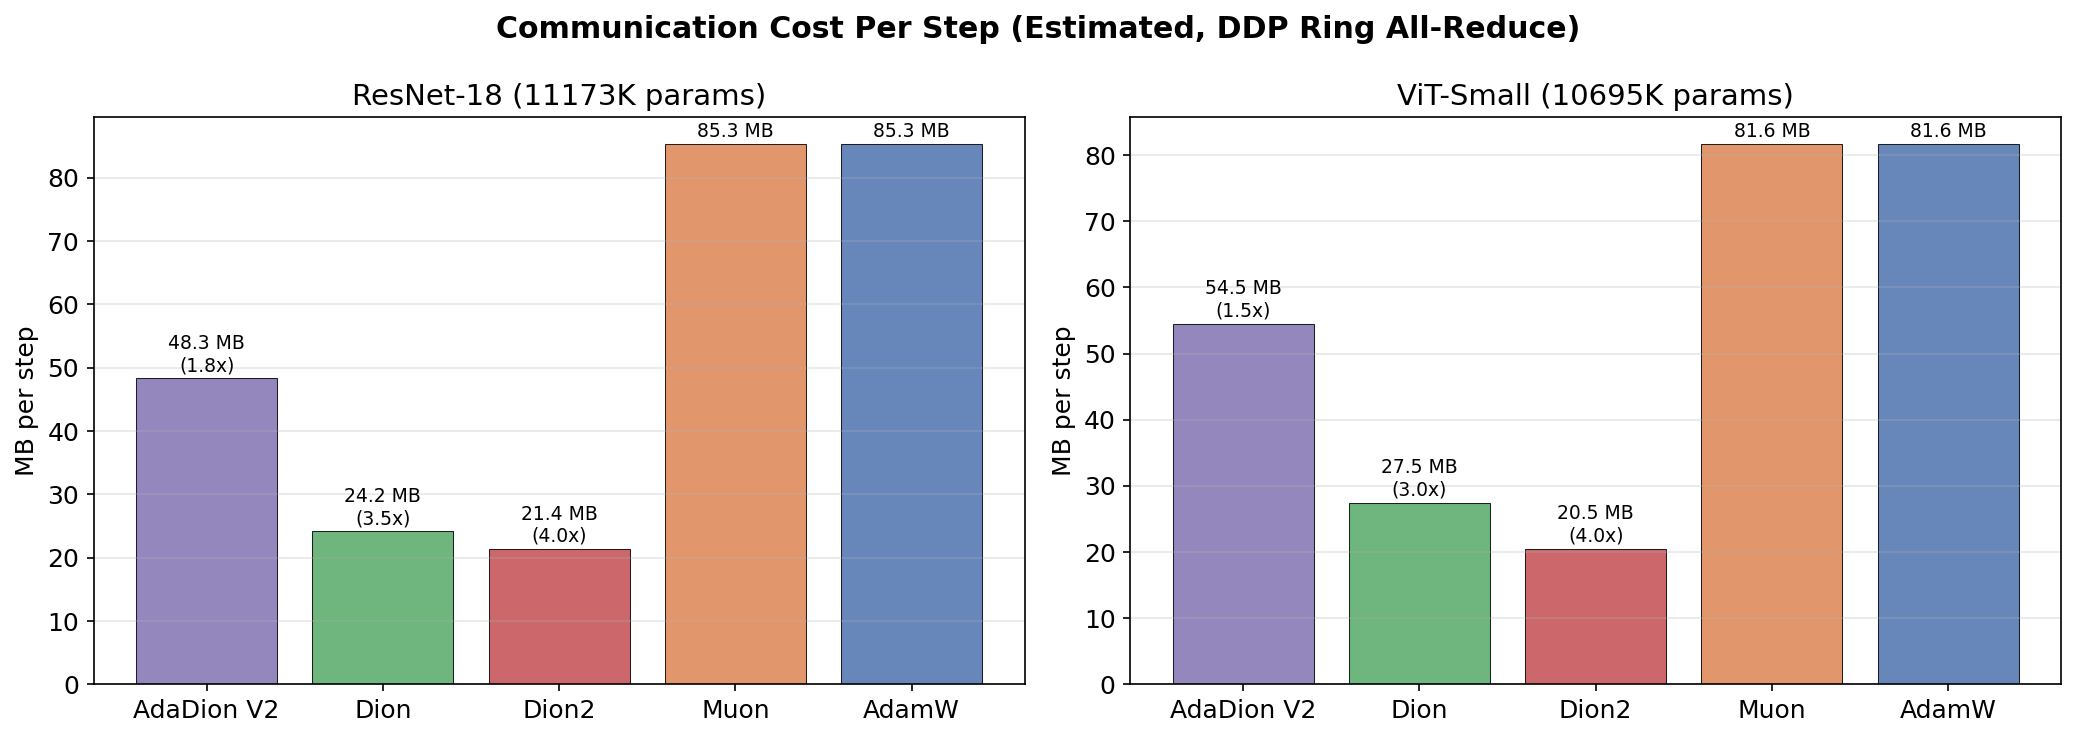
\includegraphics[width=0.95\textwidth]{figures/communication_overhead.png}
\caption{Estimated communication cost per step for each optimizer under DDP ring all-reduce. Values above bars show MB transferred and compression ratio.}
\label{fig:comm}
\end{figure*}

\section{Rank Dynamics}

\subsection{Rank and Compression}

Figure~\ref{fig:rank_tradeoff} shows the relationship between rank fraction, validation accuracy, and communication compression for AdaDion V2 on ResNet-18. Rank fraction 0.5 achieves the best accuracy (96.30\%) while still providing 1.8x compression over full all-reduce. Lower rank fractions (0.125, 0.25) provide higher compression (up to 4x) with modest accuracy loss (0.1--0.16\%). Full rank (1.0) removes compression entirely and degrades accuracy by 0.31\%, suggesting that the low-rank constraint acts as implicit regularization.

\begin{figure*}[t]
\centering
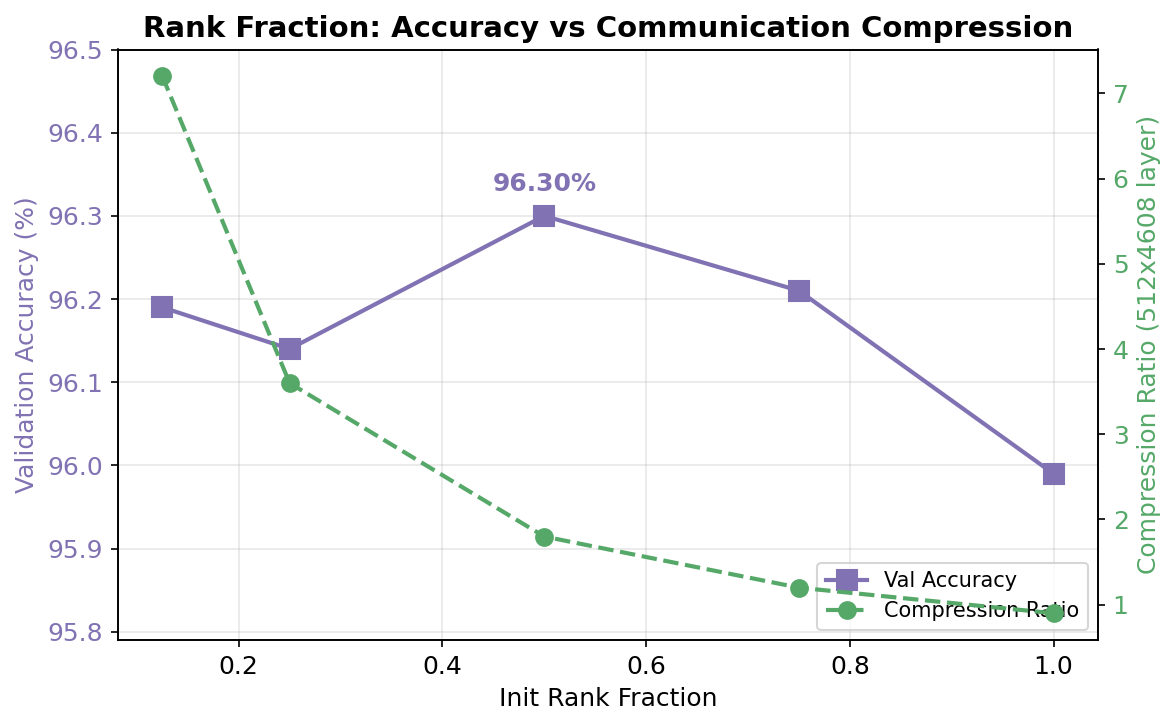
\includegraphics[width=0.85\textwidth]{figures/rank_performance_tradeoff.png}
\caption{Rank fraction vs validation accuracy (left axis) and communication compression ratio (right axis) for AdaDion V2 on ResNet-18. The optimal rank fraction (0.5) balances accuracy and compression.}
\label{fig:rank_tradeoff}
\end{figure*}

\subsection{Rank Evolution}

AdaDion V2 tracks the effective rank of each layer's gradient momentum via exponential moving average of the Shannon entropy of singular value proxies. The adaptive mechanism adjusts the active rank $r$ at each step, bounded by $[\text{rank\_min}, r_\text{cap}]$ where $r_\text{cap} = \lfloor \text{rank\_fraction\_max} \cdot \min(m, n) \rfloor$.

We tracked rank per layer across 100 epochs on ResNet-18. For the final linear layer ($10 \times 512$), $r_\text{cap} = \lfloor 0.7 \times 10 \rfloor = 7$, and the rank saturates at $r = 7$ from epoch 0 onward. This is expected: when rank\_min exceeds $r_\text{cap}$, the adaptive mechanism has no room to adjust. Rank dynamics become meaningful on larger matrices. For the flattened convolutional layers (e.g., $512 \times 4608$), $r_\text{cap} = 358$ and rank\_min $= 16$, providing a wide operating range. The ablation confirms that the optimizer benefits from this range, with rank fraction 0.5 (initializing $r \approx 256$) outperforming both lower and higher fractions.

In distributed settings, the adaptive rank introduces variable message sizes across steps. Since rank changes are rate-limited (rank\_step\_up $= 16$, rank\_step\_down $= 8$ per step) and EMA-smoothed ($\beta = 0.5$), rank transitions are gradual, limiting load imbalance in synchronous all-reduce.

\begin{figure*}[t]
\centering
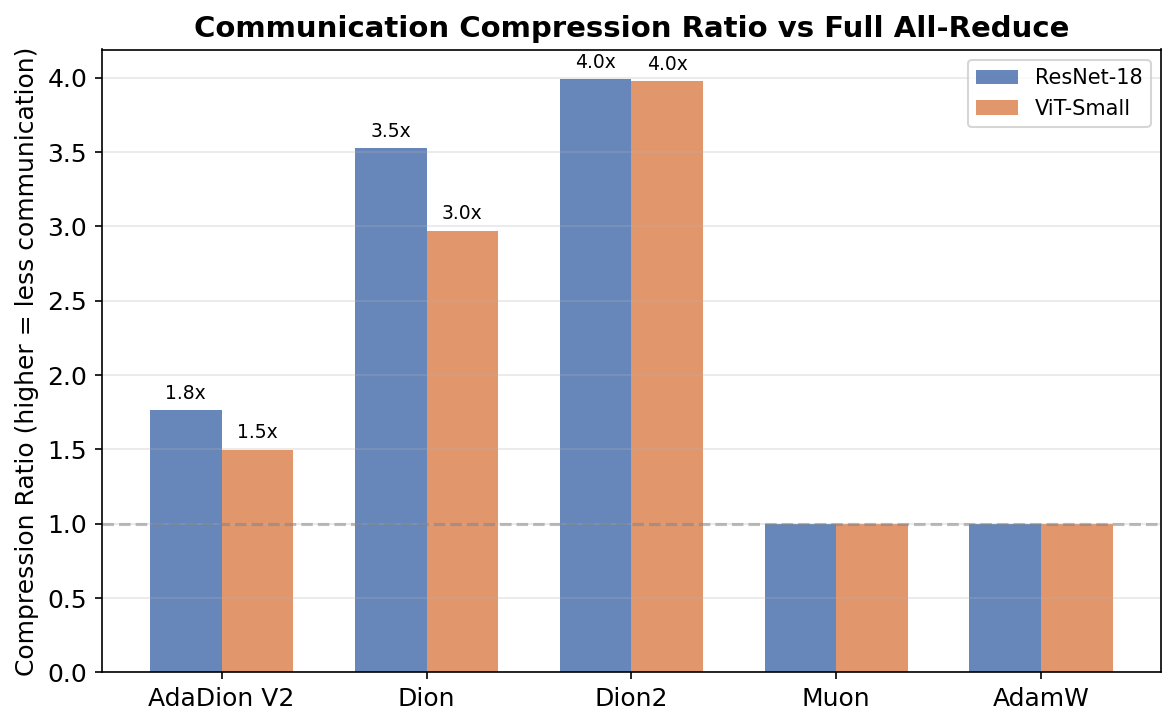
\includegraphics[width=0.85\textwidth]{figures/compression_ratio.png}
\caption{Communication compression ratio relative to full gradient all-reduce. Dion and Dion2 achieve the highest compression (3--4x). AdaDion V2 trades some compression for accuracy through its higher rank fraction.}
\label{fig:compression}
\end{figure*}

\section{Distributed Scaling}

Table~\ref{tab:comm} provides empirical 4-GPU DDP timing alongside theoretical communication estimates. Several observations follow.

\textbf{Compute overhead.} QR decomposition in Dion/AdaDion and Newton-Schulz iteration in Muon are local operations that do not scale with the number of GPUs. On 4$\times$A100, AdaDion's compute overhead is 2.8x over AdamW, while Muon's is 10.2x. As GPU count increases and communication dominates, the Dion family's overhead becomes less significant relative to the communication savings.

\textbf{Rank adaptation cost.} AdaDion V2 adds 17\% wall-clock overhead over base Dion (57.6 vs 49.4 ms/step) for effective rank estimation ($O(mr)$ column norm and entropy computation) and occasional rank resizing. This is modest relative to the $O(m^2r)$ QR decomposition.

\textbf{Scaling projection.} On bandwidth-limited interconnects (multi-node Ethernet, cross-datacenter), the 3.5x communication reduction of Dion translates directly to faster training. At 8+ GPUs on NVLink, communication overhead for AdamW and Muon grows with model size while Dion/AdaDion scale sub-linearly due to compression. The 4-GPU measurements confirm the trend: Dion is 4.2x faster than Muon despite performing comparable orthogonalization, because it communicates compressed factors rather than full gradients.

\section{Implementation Notes}
\label{sec:amp}

Adapting distributed LLM optimizers to single-GPU vision training required addressing three issues.

\textbf{Parameter coverage.}
Dion, Dion2, and AdaDion V2 reject tensors with more than 2 dimensions. On ResNet-18, 99.95\% of parameters are 4D convolutional weights. Without flattening, these optimizers operate on only the final linear layer (5,120 of 11.2M parameters). We implemented a \texttt{FlattenedParamWrapper} that reshapes 4D weights to 2D before each optimizer step and restores the original shape afterward. Without this, AdaDion V2 scored 94.95\%.

\textbf{Mixed precision.}
The spectral optimizers use \texttt{@torch.compile(fullgraph=True)} internally. When combined with \texttt{torch.amp.autocast} and \texttt{GradScaler}, float16 gradients caused graph tracing failures and silent precision loss. The fix is to run spectral optimizers in float32 without autocast or GradScaler.

\textbf{Single-GPU compatibility.}
AdaDion V2 passes \texttt{outer\_shard\_mesh} to all update functions, but the DDP code path does not accept this parameter. We conditionally pass it only for FSDP paths.

\section{Conclusion}

AdaDion V2 achieves the best validation accuracy on CIFAR-10 ResNet-18 (96.11\%) while reducing communication volume by 1.8x compared to AdamW and Muon. On 4$\times$A100 DDP, AdaDion V2 runs at 57.6 ms/step, 3.6x faster than Muon (206.3 ms/step) with higher accuracy. The adaptive rank mechanism provides 0.18\% accuracy gain over non-adaptive Dion at 17\% compute overhead. On ViT-Small, the Dion family (89.7--90.9\%) outperforms both Muon (88.8\%) and AdamW (86.2\%).

The rank-performance trade-off shows that rank fraction 0.5 balances accuracy and compression. Lower fractions (0.125--0.25) provide up to 4x communication compression with only 0.1--0.16\% accuracy loss, suitable for bandwidth-limited distributed training.

\bibliographystyle{plainnat}
\bibliography{references}

\end{document}
